\documentclass{vilniustech-en}
\vilniustechsetup{
    university={Vilnius Gediminas technical university},
    faculty={Faculty of Fundamental Sciences},
    cathedral={Department of Information Systems},
    workTitle={Malware Analysis Methods},
    workType={Laboratory Work 1},
    workAuthorName={Aurimas Šakalys},
    workAuthorGroup={ITSfm-22},
    workRecipient={lecturer Vitalijus Gurčinas}
}
\addbibresource{bibliography.bib}
\VTDocumentBegin


\section{Initial Setup}

\subsection{Laboratory Environment Setup}

\subsubsection{Malware uploading procedure}

Currently, the way that malware is introduced into the Virtual Machines are though Virtual Box Shared Folders, that are mounted within the systems. The mounts are read-only from the perspective of the Virtual Machine, which reduces the attack surface for the malware.

\begin{figure}[H]
\begin{center}
    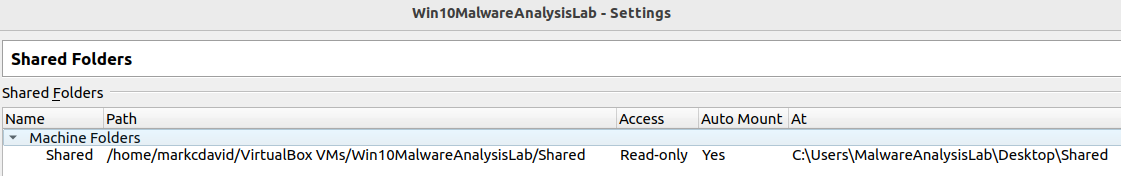
\includegraphics[width=16cm]{img/windows_shared_hyper.png}
    \caption{FLARE VM Shared Folder configuration within Virtual Box}
    \label{fig:windows_shared_hyper}
\end{center}
\end{figure}

\begin{figure}[H]
\begin{center}
    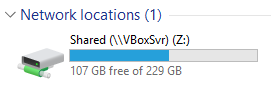
\includegraphics[width=10cm]{img/windows_shared_vm.png}
    \caption{Shared Folder within FLARE VM}
    \label{fig:windows_shared_vm}
\end{center}
\end{figure}

\begin{figure}[H]
\begin{center}
    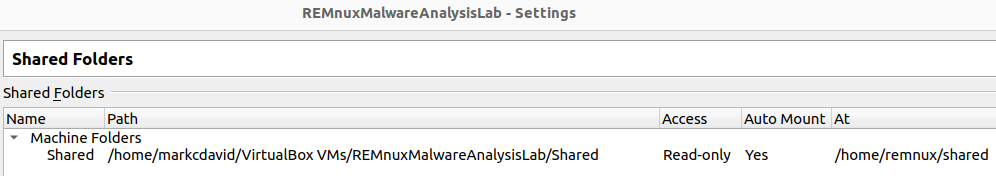
\includegraphics[width=16cm]{img/linux_shared_hyper.png}
    \caption{REMnux Shared Folder configuration within Virtual Box}
    \label{fig:linux_shared_hyper}
\end{center}
\end{figure}

\begin{figure}[H]
\begin{center}
    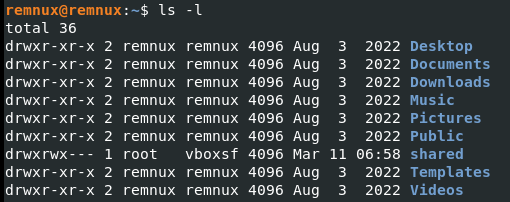
\includegraphics[width=16cm]{img/linux_shared_vm.png}
    \caption{Shared Folder within REMnux}
    \label{fig:linux_shared_vm}
\end{center}
\end{figure}

\subsubsection{Future Considerations}
While this task is mostly static analysis, where large log files and etc. are not generated, in the future we might need to extradite data from within the Virtual Machines, without providing them with an access to the internet.

Consideration is as follows - provide a host-only network, where the guest can only communicate with the host and configure the host firewall to only allow traffic that the host initiated over ssh for scp protocol to work.

I have yet to figure out how to configure this, but I think for future tasks this will be useful.

\subsection{Picking the set of malware}

We will be picking the malware from theZoo.

\textbf{More information about theZoo}

\begin{figure}[H]
\begin{center}
    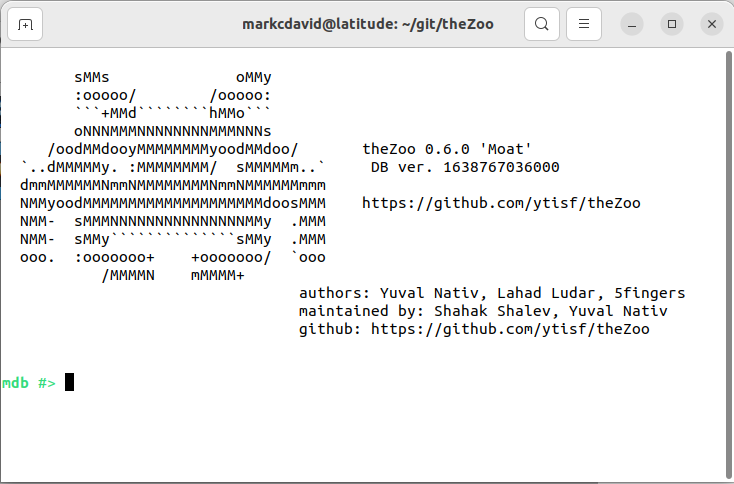
\includegraphics[width=16cm]{img/theZoo.png}
    \caption{TUI for theZoo}
    \label{fig:theZoo}
\end{center}
\end{figure}

We will pick the one virus for Linux, as it seems that theZoo could only find one malware sample for Linux. Manual checking shows that there are more samples for Linux systems within theZoo, the search simply does not show them.

\begin{figure}[H]
\begin{center}
    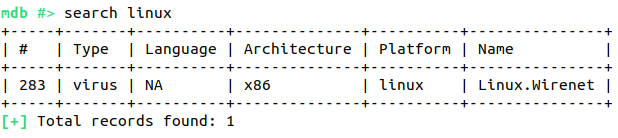
\includegraphics[width=16cm]{img/theZoo_linux.png}
    \caption{theZoo search results for Linux}
    \label{fig:theZoo_linux}
\end{center}
\end{figure}

theZoo search provides us with more malware samples for Win32 platform.

\begin{figure}[H]
\begin{center}
    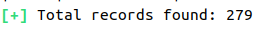
\includegraphics[width=8cm]{img/theZoo_windows.png}
    \caption{theZoo search results for Win32}
    \label{fig:theZoo_windows}
\end{center}
\end{figure}

We will choose 3 samples from this set, one worm, one trojan and one ransomware.

\begin{figure}[H]
\begin{center}
    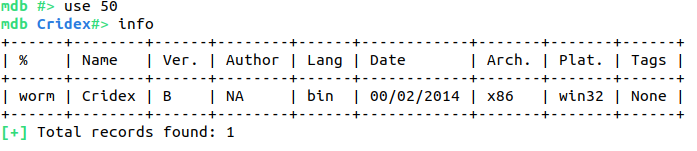
\includegraphics[width=16cm]{img/theZoo_worm.png}
    \caption{theZoo information on worm malware}
    \label{fig:theZoo_worm}
\end{center}
\end{figure}

\begin{figure}[H]
\begin{center}
    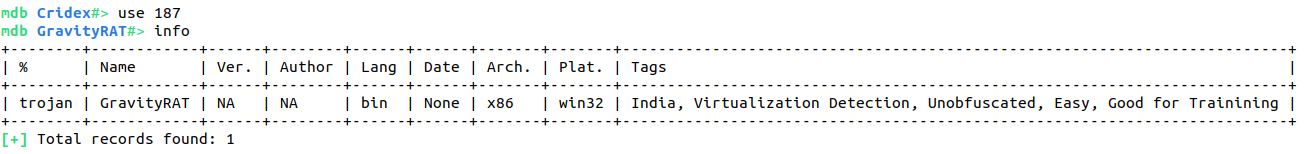
\includegraphics[width=16cm]{img/theZoo_RAT.png}
    \caption{theZoo information on troan malware}
    \label{fig:theZoo_RAT}
\end{center}
\end{figure}

\begin{figure}[H]
\begin{center}
    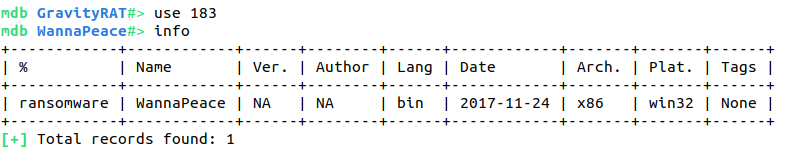
\includegraphics[width=16cm]{img/theZoo_ransom.png}
    \caption{theZoo information on ransomware malware}
    \label{fig:theZoo_ransom}
\end{center}
\end{figure}

All the samples are moved to the Virtual Machines via the shared folders.

\begin{figure}[H]
\begin{center}
    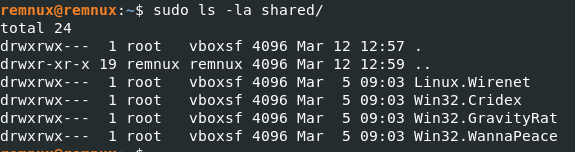
\includegraphics[width=16cm]{img/theZoo_within_linux.png}
    \caption{Malware within REMnux}
    \label{fig:theZoo_within_linux}
\end{center}
\end{figure}

\begin{figure}[H]
\begin{center}
    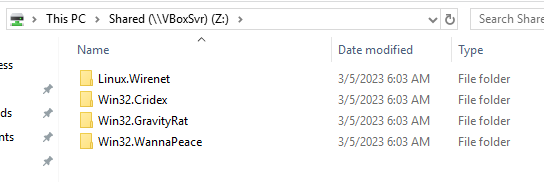
\includegraphics[width=16cm]{img/theZoo_within_windows.png}
    \caption{Malware within FLARE VM}
    \label{fig:theZoo_within_windows}
\end{center}
\end{figure}

\section{Task 1}

For malware scanning in FLARE VM we will use a free version of Malwarebytes software.

\begin{figure}[H]
\begin{center}
    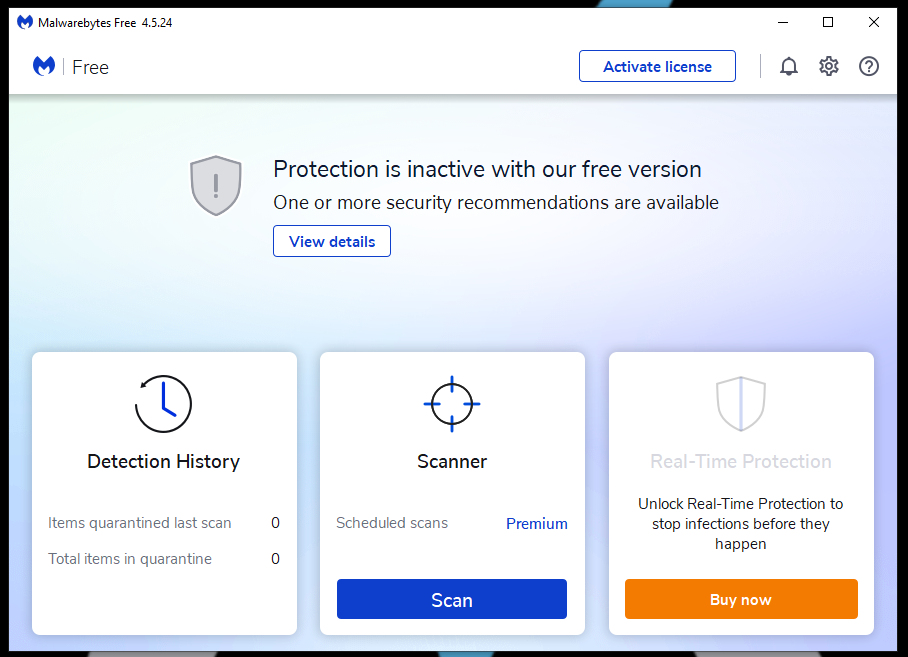
\includegraphics[width=16cm]{img/malware_bytes.png}
    \caption{Malwarebytes software}
    \label{fig:malware_bytes}
\end{center}
\end{figure}

Within REMnux, we shall use ClamAV software. Within REMnux it does not have any malware database present, as such, we need to fetch the databases using the freshclam command.
\begin{figure}[H]
\begin{center}
    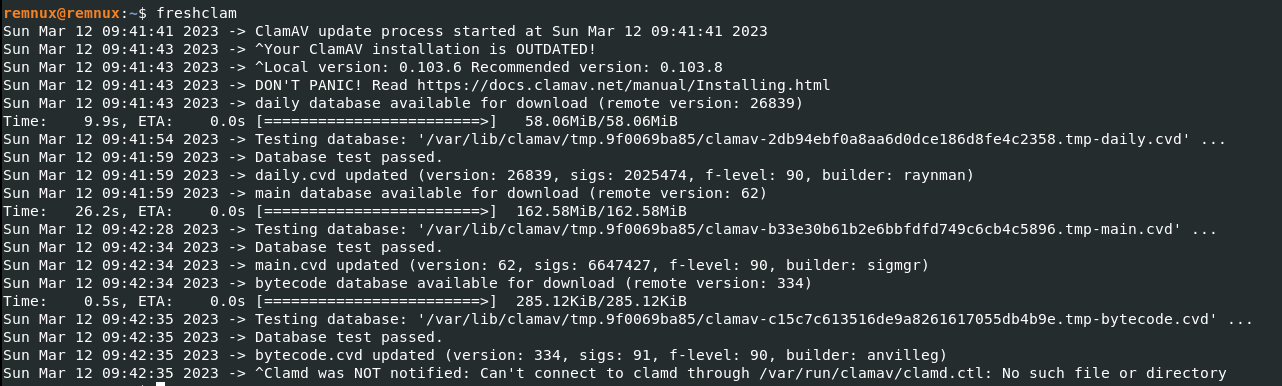
\includegraphics[width=16cm]{img/clamav.png}
    \caption{ClamAV database update}
    \label{fig:clamav}
\end{center}
\end{figure}

Although we could run clamd daemon, so that the clamscan would run a little faster, as we will not be performing a multitude of scans within the system, the performance loss is not as significant.
\begin{figure}[H]
\begin{center}
    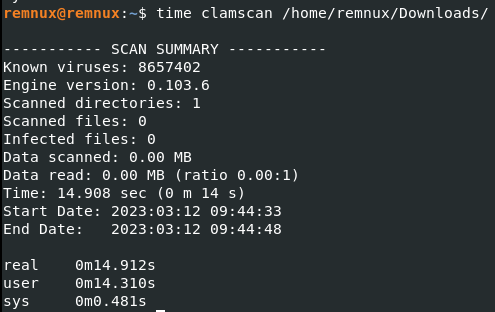
\includegraphics[width=16cm]{img/clamav_time.png}
    \caption{ClamAV database loading and scan time}
    \label{fig:clamav_time}
\end{center}
\end{figure}

\section{Task 2}

MalwareBytes has identified 3/4 malware samples, 3 of which were Windows malware, while one of them was Linux malware. All windows malware samples were identified correctly.

\begin{figure}[H]
\begin{center}
    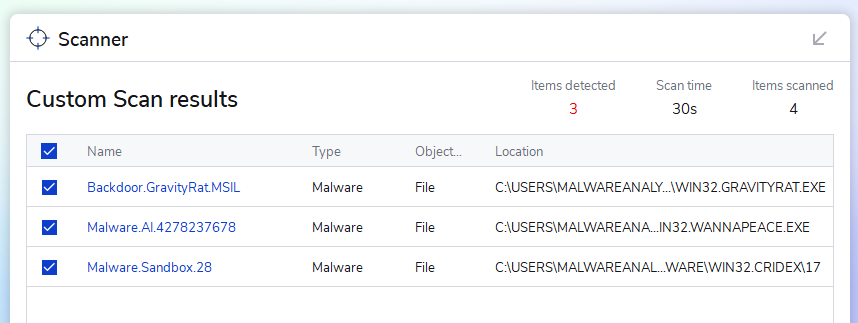
\includegraphics[width=16cm]{img/malwarebytes_scan_app.png}
    \caption{Malwarebytes scan within the application}
    \label{fig:malwarebytes_scan_app}
\end{center}
\end{figure}

\begin{figure}[H]
\begin{center}
    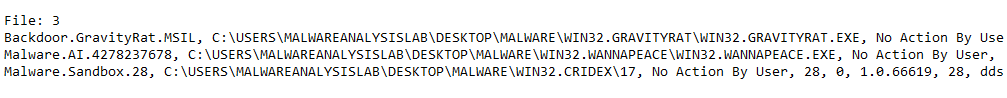
\includegraphics[width=16cm]{img/malwarebytes_scan_report.png}
    \caption{Malwarebytes scan report}
    \label{fig:malwarebytes_scan_report}
\end{center}
\end{figure}

`clamscan`, like MalwareBytes, managed to indentify 3/4 malware samples, but it identified different samples.

It did manage to identify the malware for linux system. It did miss the WannaPeace ransomware malware.

\begin{figure}[H]
\begin{center}
    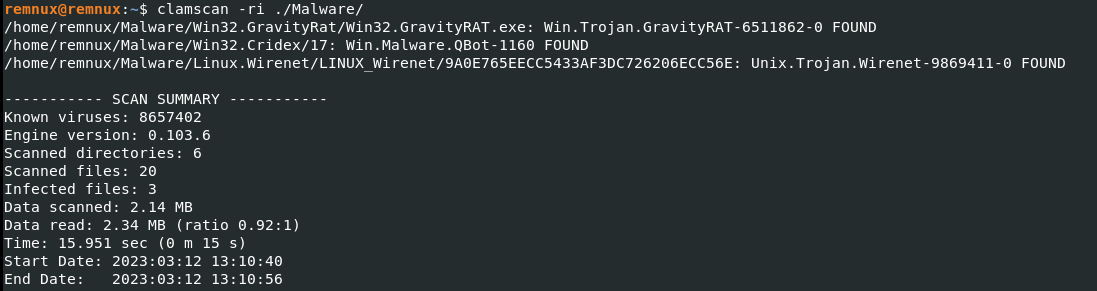
\includegraphics[width=16cm]{img/clamav_scan.png}
    \caption{ClamAV scan report}
    \label{fig:clamav_scan}
\end{center}
\end{figure}

\section{Task 3 \& Task 4}

\textbf{TASK 4 IS NOT DONE}

\textbf{TASK 4 IS NOT DONE}

\textbf{TASK 4 IS NOT DONE}

\begin{figure}[H]
\begin{center}
    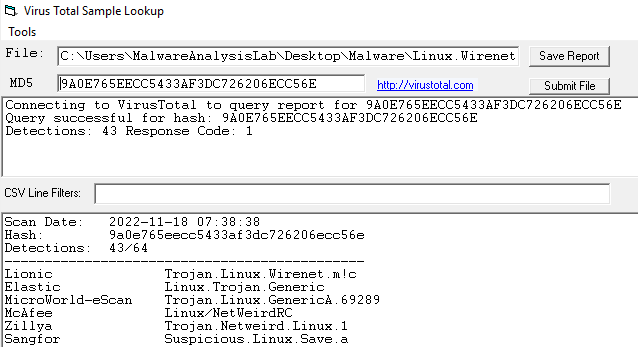
\includegraphics[width=16cm]{img/virustotal_wirenet.png}
    \caption{VirusTotal report for Linux.Wirenet}
    \label{fig:virustotal_wirenet}
\end{center}
\end{figure}

\begin{figure}[H]
\begin{center}
    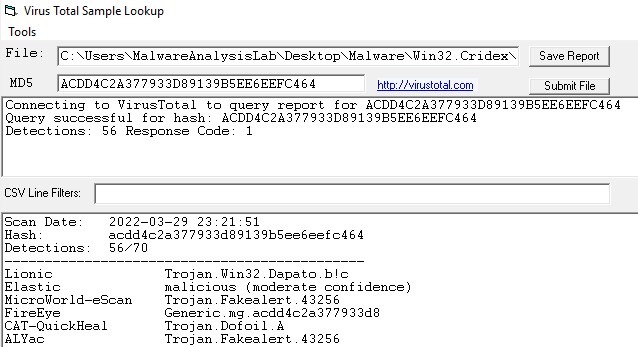
\includegraphics[width=16cm]{img/virustotal_cridex.png}
    \caption{VirusTotal report for Win32.Cridex}
    \label{fig:virustotal_cridex}
\end{center}
\end{figure}

\begin{figure}[H]
\begin{center}
    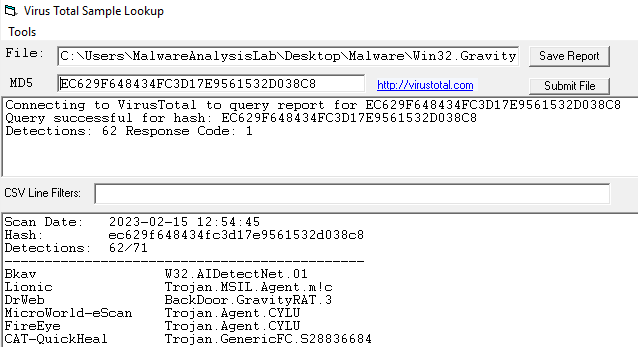
\includegraphics[width=16cm]{img/virustotal_gravityrat.png}
    \caption{VirusTotal report for Win32.GravityRAT}
    \label{fig:virustotal_gravityrat}
\end{center}
\end{figure}

\begin{figure}[H]
\begin{center}
    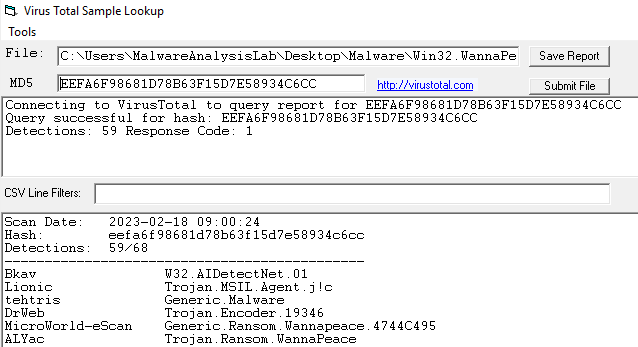
\includegraphics[width=16cm]{img/virustotal_wannapeace.png}
    \caption{VirusTotal report for Win32.WannaPeace}
    \label{fig:virustotal_wannapeace}
\end{center}
\end{figure}


\section{Task 5 \& Task 6}

Tasks 5 and 6 are combined, as we will use multiple tools in our disposal to determine possible behaviour and characteristics of the malware, that includes PE header information gathering. 

We will analyse Win32.Cridex and Win32.WannaPeace malware.

\subsection{Win32.Cridex}

First step that we will take, is to check whether the malware is packed or not. We will use peid for this.

\begin{figure}[H]
\begin{center}
    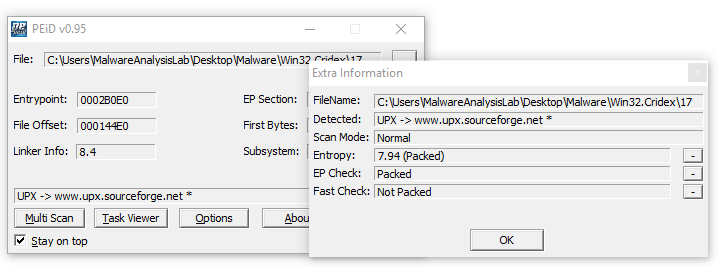
\includegraphics[width=16cm]{img/cridex_peid.png}
    \caption{peid report on Win32.Cridex}
    \label{fig:cridex_peid}
\end{center}
\end{figure}

The software provides us with the information that it has a high entropy, which is indicative of a packed malware. Additionally, it has detected, that UPX has been used to pack the software. As such, it's likely that we will be able to unpack the software.

The reason we want to unpack the software, is that we will not be able to use static analysis tools to investigate what type of behaviour the malware might have.

\begin{figure}[H]
\begin{center}
    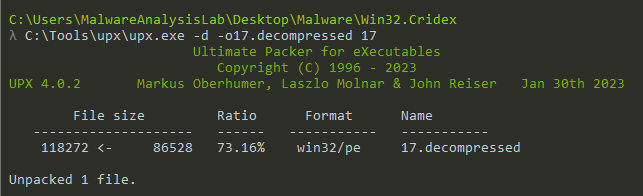
\includegraphics[width=16cm]{img/cridex_unpack.png}
    \caption{Unpacking Win32.Cridex with UPX}
    \label{fig:cridex_unpack}
\end{center}
\end{figure}

We have used UPX to unpack the malware and it worked successfully.

\begin{figure}[H]
\begin{center}
    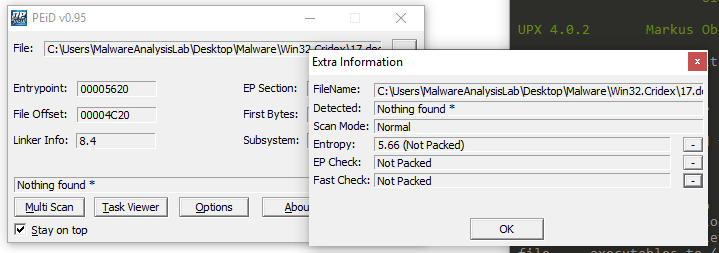
\includegraphics[width=16cm]{img/cridex_peid_unpack.png}
    \caption{peid report on Win32.Cridex after unpacking}
    \label{fig:cridex_peid_unpack}
\end{center}
\end{figure}

Getting information using `peid` we can see that the entropy had gotten down, which is indicative of software not being packed. Additionally, `peid` does not detect any packer. As such, we have malware that has been unpacked and we will not be capable of performing analysis on it's behaviour.

Using Strings we do not get much information, it seems that the malware contains a lot of randomly generated unicode strings

\begin{figure}[H]
\begin{center}
    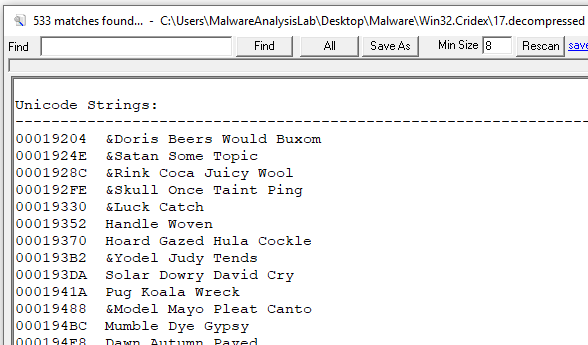
\includegraphics[width=16cm]{img/cridex_strings.png}
    \caption{strings report on unpacked Win32.Cridex}
    \label{fig:cridex_strings}
\end{center}
\end{figure}

Using CFF Explorer we can see that the malware only uses a few libraries
\begin{figure}[H]
\begin{center}
    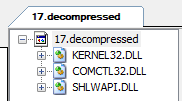
\includegraphics[width=10cm]{img/cridex_cff.png}
    \caption{CFF Explorer dependency report on unpacked Win32.Cridex}
    \label{fig:cridex_cff}
\end{center}
\end{figure}

To make our work a bit easier, we will use Ghidra to analyse the malware and provide us with the functions calls to these libraries. Using these we could determine a few characteristics about the malware.

Ghidra, after analysing the malware, shows us that the malware uses `LoadLibraryW` and `LoadLibraryExW` API calls.
\begin{figure}[H]
\begin{center}
    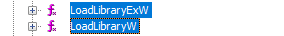
\includegraphics[width=10cm]{img/cridex_ghidra.png}
    \caption{Ghida report on used API calls in unpacked Win32.Cridex}
    \label{fig:cridex_ghidra}
\end{center}
\end{figure}

This means that the Malware could possibly dynamically load libraries and this does not provide an indication as to what the behaviour of the malware is. The next steps would be to either do reverse engineering or perform dynamic analysis and run the sample. We shall skip these steps for now.

\subsection{Win32.WannaPeace}

We shall run a similar procedure for the WannaPeace malware.

Using `peid` we can find an indication, that the malware is packed. 

\begin{figure}[H]
\begin{center}
    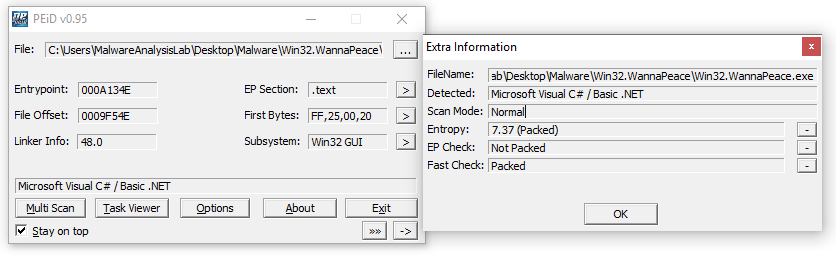
\includegraphics[width=16cm]{img/wannapeace_peid.png}
    \caption{peid report on Win32.WannaPeace}
    \label{fig:wannapeace_peid}
\end{center}
\end{figure}

Additionally, we can see an indication that this is a .NET executable, which should allow us to try to analyse the malware using `dnSpy`. 

\begin{figure}[H]
\begin{center}
    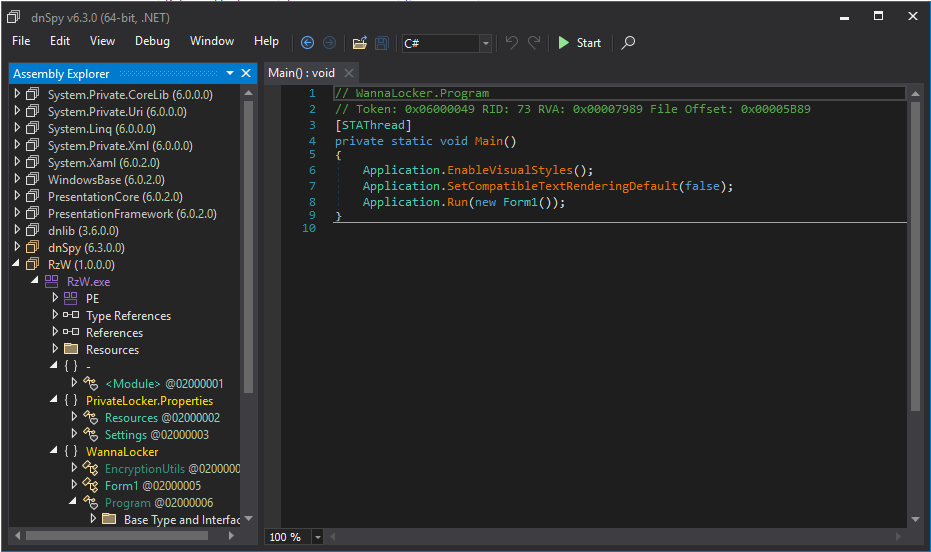
\includegraphics[width=16cm]{img/wannapeace_dnspy_main.png}
    \caption{Main function of Win32.WannaPeace}
    \label{fig:wannapeace_dnspy_main}
\end{center}
\end{figure}

We can see that the malware is a WinForms application. The `Main` method simply creates the new form and that would seem to be the entire functionality.

\begin{figure}[H]
\begin{center}
    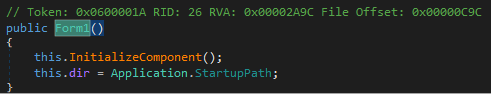
\includegraphics[width=16cm]{img/wannapeace_dnspy_form_init.png}
    \caption{Main form initialisation of Win32.WannaPeace}
    \label{fig:wannapeace_dnspy_form_init}
\end{center}
\end{figure}

We are partially cheating here, as we do know this is a ransomware type of malware, as such, we would expect the users' filesystem to be encrypted prior to the execution of the form that asks for the ransom. Where would we be able to find it?

We can find a namespace/class for encryption utilities, and it has functions for encrypting files and directories. 

\begin{figure}[H]
\begin{center}
    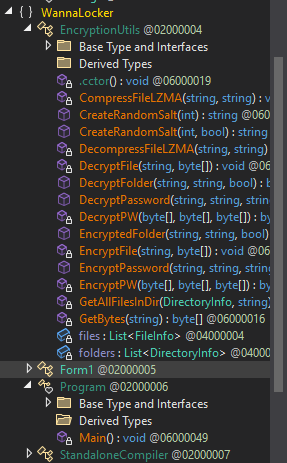
\includegraphics[width=10cm]{img/wannapeace_dnspy_crypto.png}
    \caption{Cryptographic helper functions of Win32.WannaPeace}
    \label{fig:wannapeace_dnspy_crypto}
\end{center}
\end{figure}

We want to determine, where the usage of these functions begin. If we look at the usages of `EncryptFolder` function,
we can see that it is used from a `bgw\_DoWork` method. 

\begin{figure}[H]
\begin{center}
    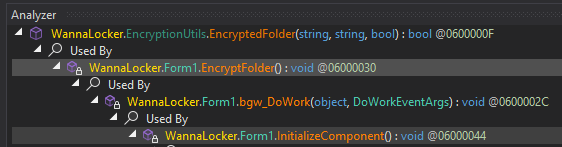
\includegraphics[width=16cm]{img/wannapeace_bgw.png}
    \caption{Usage tree for EncryptFolder function in Win32.WannaPeace}
    \label{fig:wannapeace_bgw}
\end{center}
\end{figure}

`bgw`, usually stands for `BackGround Worker`, and the `DoWork` postfix provides us some indication that this might be true. 


\begin{figure}[H]
\begin{center}
    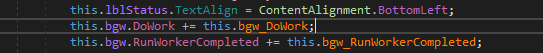
\includegraphics[width=16cm]{img/wannapeace_bgw_subscribe.png}
    \caption{Background worker method subscription in Win32.WannaPeace}
    \label{fig:wannapeace_bgw_subscribe}
\end{center}
\end{figure}

\begin{figure}[H]
\begin{center}
    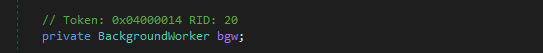
\includegraphics[width=16cm]{img/wannapeace_bgw_store.png}
    \caption{Background worker variable in Win32.WannaPeace}
    \label{fig:wannapeace_bgw_store}
\end{center}
\end{figure}

\begin{figure}[H]
\begin{center}
    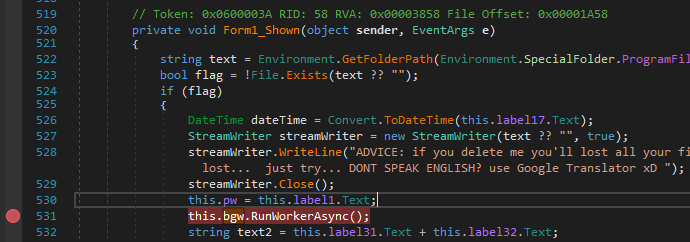
\includegraphics[width=16cm]{img/wannapeace_bgw_usage.png}
    \caption{Usage of the background worker in Win32.WannaPeace}
    \label{fig:wannapeace_bgw_usage}
\end{center}
\end{figure}

We can see that the background worker is created during composition of the form and when the form is first shown it launches the worker, which in turn - encrypts the users file.

`bgw2\_DoWork` launches the decryption algorithm, but it only launches if user provides correct password for the decryption.

\begin{figure}[H]
\begin{center}
    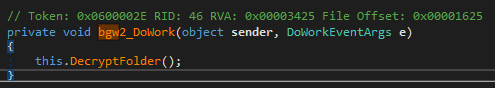
\includegraphics[width=16cm]{img/wannapeace_bgw2.png}
    \caption{Subsciption method for second background worker in Win32.WannaPeace}
    \label{fig:wannapeace_bgw2}
\end{center}
\end{figure}

\begin{figure}[H]
\begin{center}
    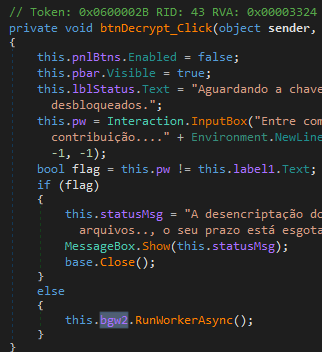
\includegraphics[width=10cm]{img/wannapeace_bgw2_usage.png}
    \caption{Behaviour code for second background worker in Win32.WannaPeace}
    \label{fig:wannapeace_bgw2_usage}
\end{center}
\end{figure}

\section{Task 7}

We will use In Shadow Batch Virus Generator to generate our malware.


\begin{figure}[H]
\begin{center}
    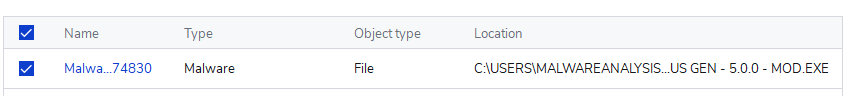
\includegraphics[width=16cm]{img/malware_gen_scan.png}
    \caption{Malwarebytes scan result for In Shadow Batch Virus Generator}
    \label{fig:malware_gen_scan}
\end{center}
\end{figure}

The generator itself is being marked as malware. `peid` provides us with information, that this is a .NET executable, which means we could check for untoward behaviour with `dnSpy` as well.

\begin{figure}[H]
\begin{center}
    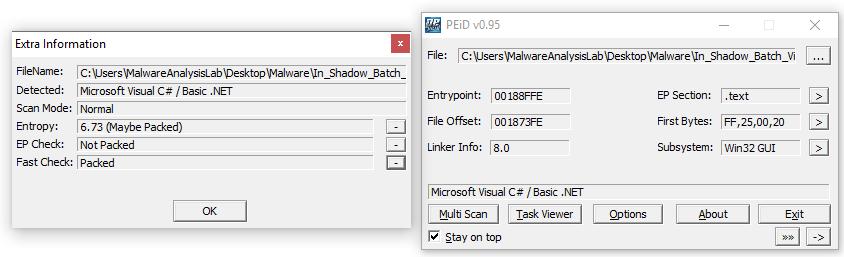
\includegraphics[width=16cm]{img/malware_gen_peid.png}
    \caption{peid report on In Shadow Batch Virus Generator}
    \label{fig:malware_gen_peid}
\end{center}
\end{figure}

A quick analysis using `dnSpy` shows that the software does not seem to be malicous and at most it simply generates a batch file using snippets within resources or code itself.
As the software is deemed safe to use, we shall proceed.

\begin{figure}[H]
\begin{center}
    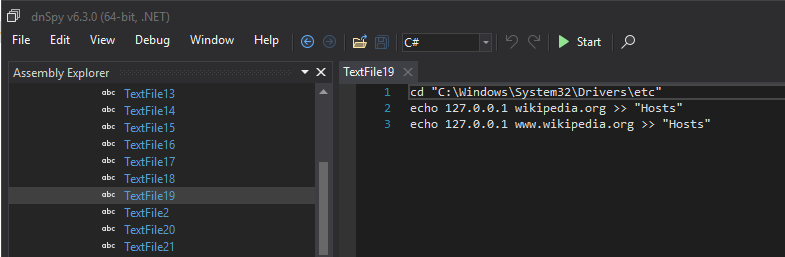
\includegraphics[width=16cm]{img/malware_gen_resource.png}
    \caption{Resources file within In Shadow Batch Virus Generator}
    \label{fig:malware_gen_resource}
\end{center}
\end{figure}


\begin{figure}[H]
\begin{center}
    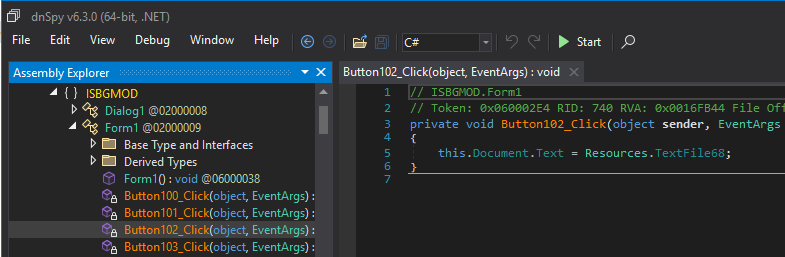
\includegraphics[width=16cm]{img/malware_gen_behaviour.png}
    \caption{Behaviour of a button click function within In Shadow Batch Virus Generator}
    \label{fig:malware_gen_behaviour}
\end{center}
\end{figure}


\subsection{Fun Aside}
Apparantly, this software has easter eggs within it. As Easter Eggs are considered to be malicious, this software could now be classified as malware.

\begin{figure}[H]
\begin{center}
    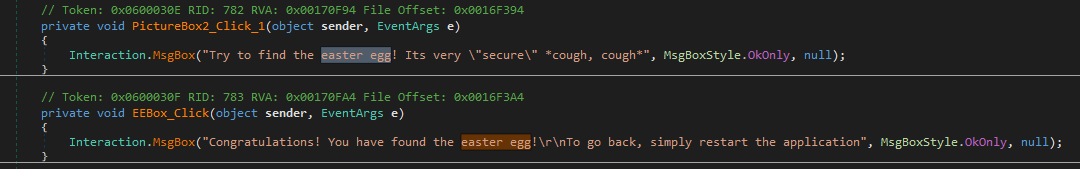
\includegraphics[width=16cm]{img/malware_gen_easter_egg.png}
    \caption{Indication of an easter egg within In Shadow Batch Virus Generator}
    \label{fig:malware_gen_easter_egg}
\end{center}
\end{figure}

\subsection{Generated Malware}
Using the generator, a sample malicous batch file has been created. 
\begin{figure}[H]
\begin{center}
    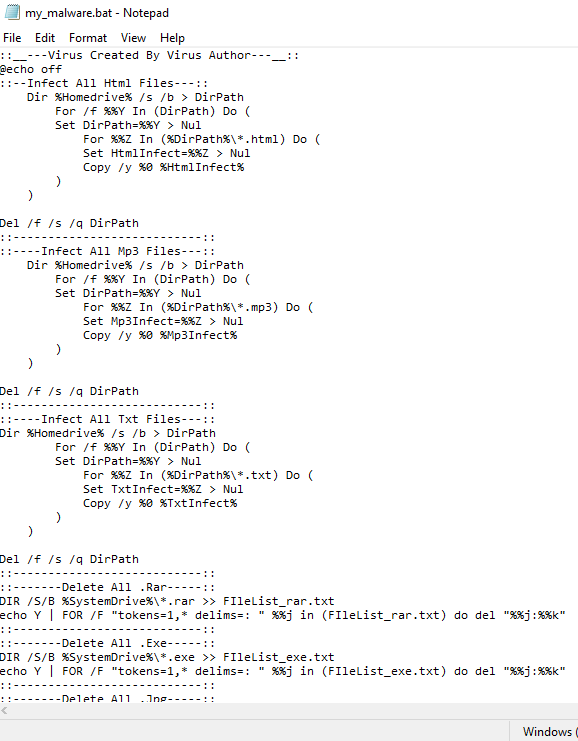
\includegraphics[width=16cm]{img/generated_malware.png}
    \caption{Generated batch file malware}
    \label{fig:generated_malware}
\end{center}
\end{figure}

Additionally, Malwarebytes does not detect it as a malicous software.
\begin{figure}[H]
\begin{center}
    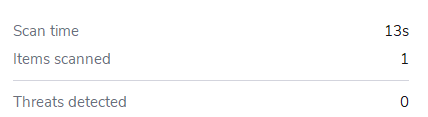
\includegraphics[width=16cm]{img/malwarebytes_generated_scan.png}
    \caption{Scan of the generated batch malware}
    \label{fig:malwarebytes_generated_scan}
\end{center}
\end{figure}

\section{Task 8}

For this task, we shall cheat a little, and use a Cridex malware sample that we decompressed in Task 5/6. We can check, that both the compressed and decompressed malware is detected by Malwarebytes.  

\begin{figure}[H]
\begin{center}
    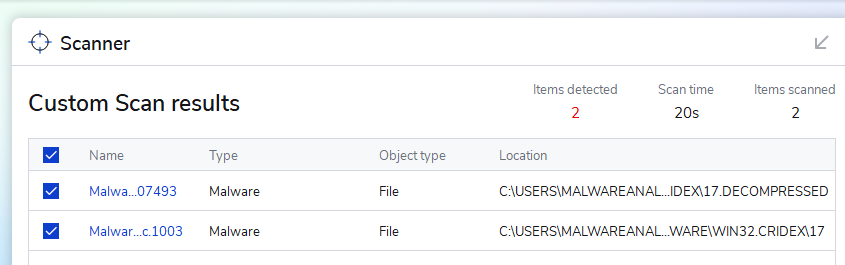
\includegraphics[width=16cm]{img/mawlarebytes_scan_unpacked.png}
    \caption{Scan of Win32.Cridex malware}
    \label{fig:mawlarebytes_scan_unpacked}
\end{center}
\end{figure}

We have used UPX to pack the file. We can see that the file now has a similar size. Let's check the hashes of the files to ensure that we have not created the exact same files.

\begin{figure}[H]
\begin{center}
    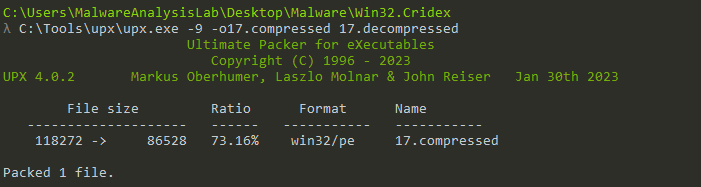
\includegraphics[width=16cm]{img/packing_process_max_compression.png}
    \caption{Packing of the Win32.Cridex malware}
    \label{fig:packing_process_max_compression}
\end{center}
\end{figure}

\begin{figure}[H]
\begin{center}
    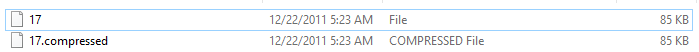
\includegraphics[width=16cm]{img/packing_similar_size.png}
    \caption{Indication of similar sized executables}
    \label{fig:packing_similar_size}
\end{center}
\end{figure}

HashMyFiles software provides us with hashes for both malware and we can see that it is indeed different. 

\begin{figure}[H]
\begin{center}
    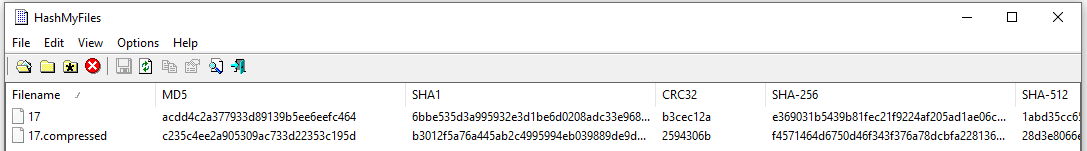
\includegraphics[width=16cm]{img/packing_hash.png}
    \caption{Hash of packed malware}
    \label{fig:packing_hash}
\end{center}
\end{figure}
If it had been the same, we could have used a different level of compression via UPX (e.g. -1 instead of -9), to get a less compressed, but different file.

\begin{figure}[H]
\begin{center}
    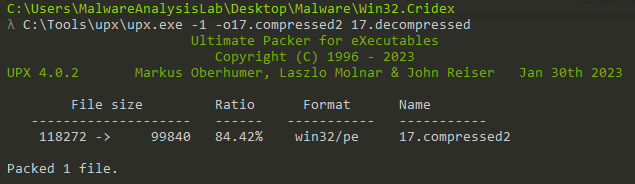
\includegraphics[width=16cm]{img/packing_process_min_compression.png}
    \caption{Packing process with smaller compression rate}
    \label{fig:packing_process_min_compression}
\end{center}
\end{figure}

\begin{figure}[H]
\begin{center}
    \includegraphics[width=16cm]{img/packing_size_hash.png}
    \caption{Hashes of differently packed malware}
    \label{fig:packing_size_hash}
\end{center}
\end{figure}

As we can see, after rescanning the malware samples, the newly packed malware samples are not detected anymore by Malwarebytes.

\begin{figure}[H]
\begin{center}
    \includegraphics[width=16cm]{img/scan_of_repacked_malware.png}
    \caption{Scan of packed malware}
    \label{fig:scan_of_repacked_malware}
\end{center}
\end{figure}

\section{Task 9}

For this task, we shall use Cuckoo Sandbox, that is hosted online. We can find one like this at `cuckoo.cert.ee`. This allows us to forgoe (for now) the need to set up the sandbox ourselves, and will provide us with required data.

We shall analyse Win32.GravityRAT and Win32.WannaPeace malware using Cuckoo Sandbox.

\begin{figure}[H]
\begin{center}
    \includegraphics[width=16cm]{img/cuckoo_wannapeace_scan.png}
    \caption{Cuckoo sandbox scan of Win32.WannaPeace malware}
    \label{fig:cuckoo_wannapeace_scan}
\end{center}
\end{figure}

\begin{figure}[H]
\begin{center}
    \includegraphics[width=16cm]{img/cuckoo_rat_scan.png}
    \caption{Cuckoo sandbox scan of Win32.GravityRAT malware}
    \label{fig:cuckoo_rat_scan}
\end{center}
\end{figure}

We can see the results for both of these malware samples. They scored 10/10, which shows that this malware is extremelly suspicious.

\begin{figure}[H]
\begin{center}
    \includegraphics[width=16cm]{img/malware_sus.png}
    \caption{Suspicion rating for provided malware}
    \label{fig:malware_sus}
\end{center}
\end{figure}

\subsection{Win32.WannaPeace}

Cuckoo is capable of providing a lot of information that we would collect in one area (PE headers, section sizes, entropy etc.). While these could be useful for analysis, the sandbox provides a summary of actions and behaviours taken by the malware.

\begin{figure}[H]
\begin{center}
    \includegraphics[width=16cm]{img/cuckoo_peace_results.png}
    \caption{Results of Cuckoo sandbox analysis for Win32.WannaPeace malware}
    \label{fig:cuckoo_peace_results}
\end{center}
\end{figure}

To begin, this shows an inexperienced malware analyst certain behavioral patterns, that could be useful for future malware analysis efforts (e.g. checking for total memory using `GlobalMemoryStatusEx` to detect virtual machines with low memory). 

As we can see in the results above, a lot of indication for suspicion of the file is that it is detected by the malware scanners, not from the behaviour.

It is shown as a packed malware, when in truth it is simply a .NET CLR executable, which shows up as packed due to high file entropy.

Cuckoo was unable to determine, by behavioral analysis the severity of the malware.

\subsection{Win32.GravityRAT}

The results are a bit different with the GravityRAT malware, as it triggers a few more rules within the Cuckoo Sandbox.

\begin{figure}[H]
\begin{center}
    \includegraphics[width=16cm]{img/cuckoo_rat_results.png}
    \caption{Results of Cuckoo sandbox analysis for Win32.GravityRAT malware}
    \label{fig:cuckoo_rat_results}
\end{center}
\end{figure}

The malware exibits a bit more suspicious behaviour, like moving it's own executable to a new location, tries harder to detect if it was ran within a virtual machine and actually sent data back to CnC. 

We can determine that (desipte knowing that the malware is a RAT) the malware is capable of obfuscating and hiding itself within the system, sending out data back to CnC, indicating it's a RAT.

\VTDocumentEnd